\section{Atomic Structure} % Source 110, 125

\begin{multicols}{2}


\section*{The Atom}


\subsection{Dalton's Model}

\begin{center}
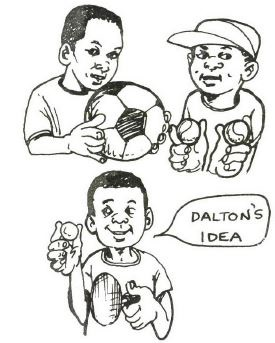
\includegraphics[width=0.4\textwidth]{./img/source/dalton-model.jpg}
\end{center}

\begin{description*}
%\item[Subtopic:]{}
\item[Materials:]{Football, orange, balls of other sizes}
%\item[Setup:]{}
\item[Theory:]{Dalton stated that atoms are round and
that the atoms of different elements ale not alike
in diameter and chemical properties. }
\item[Procedure:]{Let students bring balls of different diameters
made from different materials. Let them discuss
these models and their shortcomings.}
%\item[Hazards:]{}
%\item[Questions:]{}
%\item[Observations:]{}
%\item[Applications:]{}
%\item[Notes:]{}
\end{description*}

\subsection{Atom Model Displays}

\begin{center}
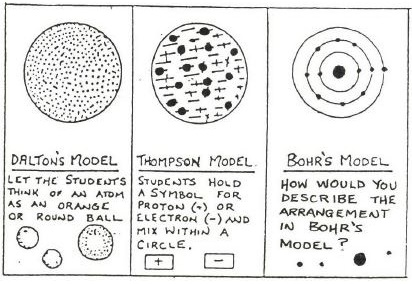
\includegraphics[width=0.45\textwidth]{./img/source/models-atom-str-alt.jpg}
\end{center}

\begin{description*}
%\item[Subtopic:]{}
\item[Materials:]{Manila paper, bamboo sticks, string, paper, marker pens}
%\item[Setup:]{}
\item[Procedure:]{Prepare display charts for the different atomic models developed throughout history (Dalton, Thompson, Rutherford).}
%\item[Hazards:]{}
%\item[Questions:]{}
%\item[Observations:]{}
%\item[Theory:]{}
%\item[Applications:]{}
%\item[Notes:]{}
\end{description*}

\columnbreak

\subsection{Particle Packing}

\begin{center}
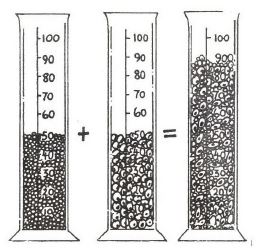
\includegraphics[width=0.35\textwidth]{./img/source/dalton-measure.jpg}
\end{center}

\begin{description*}
%\item[Subtopic:]{}
\item[Materials:]{Measuring cylinders, sand, seeds/stones}
%\item[Setup:]{}
\item[Procedure:]{Mix 50 ml of fine sand with 50 ml of seeds
or stones.}
%\item[Hazards:]{}
\item[Questions:]{What is the resulting volume?}
\item[Observations:]{The resulting volume is less than 100 ml.}
\item[Theory:]{The small molecules are able to fill the space
between the larger molecules. The greater the
difference in size, the greater the volume decrease
is. This provides a better understanding of
Dalton's model.}
%\item[Applications:]{}
%\item[Notes:]{}
\end{description*}

%==================================================================================================%

\section*{Electron Arrangements}


\subsection{Student Atoms}

\begin{center}
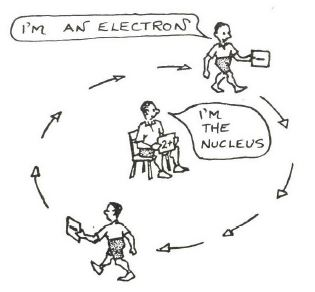
\includegraphics[width=0.4\textwidth]{./img/source/student-atom.jpg}
\end{center}

\begin{description*}
%\item[Subtopic:]{}
\item[Materials:]{Balloons or cards/papers, markers}
%\item[Setup:]{}
\item[Procedure:]{Give each student a card or balloon with a different symbol written on it (`+' for proton, `-' for electron, blank for neutron). Students arrange themselves to show a particular atom. Draw circles with chalk on the ground to represent different electron shells.}
%\item[Hazards:]{}
%\item[Questions:]{}
%\item[Observations:]{}
%\item[Theory:]{}
%\item[Applications:]{}
%\item[Notes:]{}
\end{description*}

\subsection{Models of Atoms}

\begin{center}
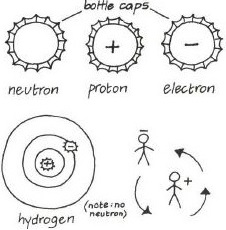
\includegraphics[width=0.32\textwidth]{./img/vso/atom-model.jpg}
\end{center}

\begin{description*}
%\item[Subtopic:]{}
\item[Materials:]{Bottle caps, marker}
%\item[Setup:]{}
\item[Procedure:]{Label bottle caps at protons (`+'), electrons (`-') and neutrons (blank). Create models for different atoms by placing the appropriate number of protons and neutrons in the center (nucleus) and electrons on drawn circles around the outside. Draw circles on desks or
floors to represent the electron
shells. }
%\item[Hazards:]{}
%\item[Questions:]{}
%\item[Observations:]{}
\item[Theory:]{All atoms contain a nucleus
(protons and neutrons) and
electrons found in different shells around the nucleus. }
%\item[Applications:]{}
\item[Notes:]{Alternatively use students
to represent the electron shells.}
\end{description*}

\subsection{Size of the Nucleus}

\begin{center}
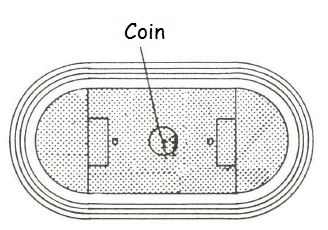
\includegraphics[width=0.4\textwidth]{./img/source/size-nucleus.jpg}
\end{center}

\begin{description*}
%\item[Subtopic:]{}
%\item[Materials:]{}
%\item[Setup:]{}
%\item[Procedure:]{}
%\item[Hazards:]{}
%\item[Questions:]{}
\item[Observations:]{Ask students to imagine how small the
nucleus is compared with the size of the whole
atom by thinking of the following comparison.
If an atom could be magnified to the size of the
National Stadium in Dar es Salaam, then the
nucleus would have the size of one coin
placed on the centre spot. The rest of the atom is
just empty space in which the electrons move
haphazardly.}
%\item[Theory:]{}
%\item[Applications:]{}
%\item[Notes:]{}
\end{description*}

\columnbreak

\subsection{Atoms on the Ground}

\begin{center}
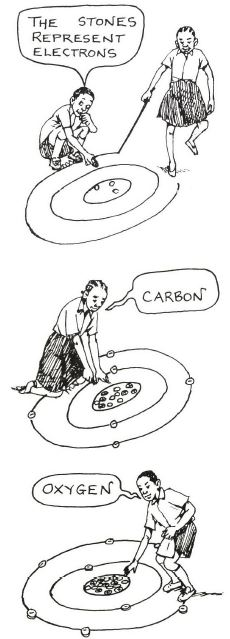
\includegraphics[width=0.4\textwidth]{./img/source/stone-atoms.jpg}
\end{center}

\begin{description*}
%\item[Subtopic:]{}
\item[Materials:]{Bottle caps or stones, string}
%\item[Setup:]{}
\item[Procedure:]{Lay string in circles on the ground to represent the electron shells. Place marked stones or bottle caps to represent protons, neutrons and electrons and construct different atoms.}
%\item[Hazards:]{}
%\item[Questions:]{}
%\item[Observations:]{}
%\item[Theory:]{}
%\item[Applications:]{}
%\item[Notes:]{}
\end{description*}

\vfill
\columnbreak

%==================================================================================================%

\section*{Electron Arrangements}


\subsection{Dormitory Model}

\begin{center}
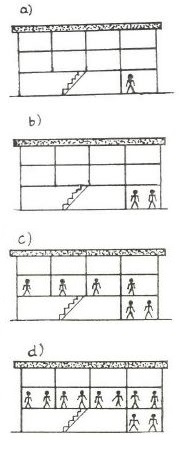
\includegraphics[width=0.4\textwidth]{./img/source/dorm-arrangement.jpg}
\end{center}

\begin{description*}
%\item[Subtopic:]{}
%\item[Materials:]{}
%\item[Setup:]{}
\item[Procedure:]{Imagine a school has a dormitory with one room on the
ground floor, four rooms on the first floor and
four rooms on the second floor. The house
master has stated that each room must be occupied by two students. However, upper rooms cannot be occupied until all lower rooms are filled. Pairing only occurs when each room on that floor has at least one student.}
%\item[Hazards:]{}
%\item[Questions:]{}
%\item[Observations:]{}
\item[Theory:]{This is the same way in which electrons fill electron shells, or energy levels. This configuration is the most stable for electrons.}
%\item[Applications:]{}
%\item[Notes:]{}
\end{description*}

\vfill
\columnbreak

\subsection{Shelf Model}

\begin{center}
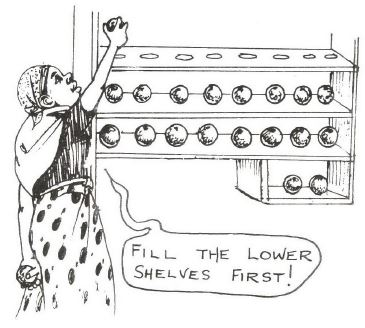
\includegraphics[width=0.38\textwidth]{./img/source/shelf-model.jpg}
\end{center}

\begin{description*}
%\item[Subtopic:]{}
%\item[Materials:]{}
%\item[Setup:]{}
%\item[Procedure:]{}
%\item[Hazards:]{}
%\item[Questions:]{}
\item[Observations:]{}
\item[Theory:]{This is an alternative to the school dormitory
model. The rules are similar. The upper shelves cannot be occupied until all
the lower shelves are occupied by oranges.
This is a simpler model since it does not
involve the pairing principle.}
%\item[Applications:]{}
%\item[Notes:]{}
\end{description*}

%==================================================================================================%

\section*{Isotopes}


\subsection{Isotope Models}

\begin{center}
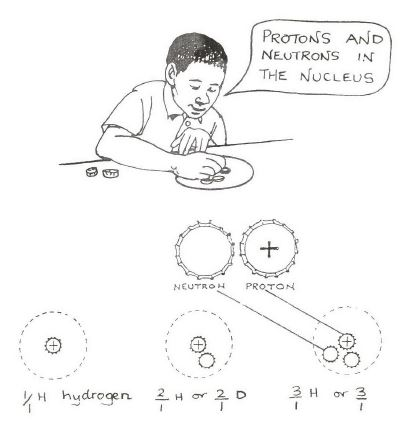
\includegraphics[width=0.45\textwidth]{./img/source/isotopes.jpg}
\end{center}

\begin{description*}
%\item[Subtopic:]{}
\item[Materials:]{Bottle caps}
%\item[Setup:]{}
\item[Procedure:]{Cut a large
circle from a piece of card to represent
the nucleus of an atom. Use bottle caps to represent protons and
neutrons. Leave some caps blank
for neutrons and mark others `+' for protons.
Place bottle caps to show protons and neutrons of some
isotopes of hydrogen, oxygen, carbon etc.}
%\item[Hazards:]{}
%\item[Questions:]{}
%\item[Observations:]{}
\item[Theory:]{\emph{Isotopes} are atoms of the same element with the same number of protons but different numbers of neutrons. Isotopes of hydrogen are shown.}
%\item[Applications:]{}
%\item[Notes:]{}
\end{description*}

%==================================================================================================%


\end{multicols}

\pagebreak